% LTeX: language=it

\section{Spettro elettromagnetico}

Lo spettro elettromagnetico è l'insieme delle frequenze delle onde elettromagnetiche.
É possibile suddividere lo spettro elettromagnetico in sette grandi categorie:

\begin{figure}[H]
    \centering
    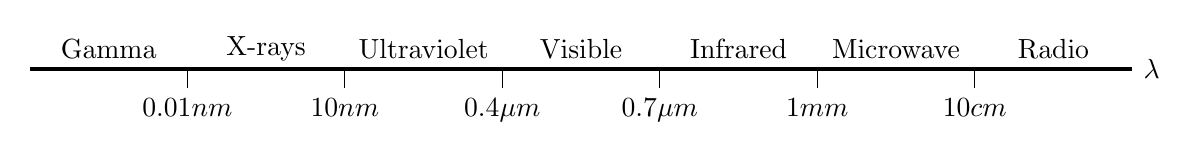
\begin{tikzpicture}[scale=0.5]
        % Spectrum lines
        \draw[ultra thick] (0,0) -> (28,0) node[right] {$\lambda$};

        % Wavelengths
        \foreach \w/\label in {4/$0.01nm$, 8/$10nm$, 12/$0.4\mu m$, 16/$0.7\mu m$, 20/$1mm$, 24/$10cm$}
            {
                \draw (\w,0) -- (\w,-0.5) node[below] {\label};
            }

        % Labels
        \foreach \w/\label in {2/Gamma, 6/X-rays, 10/Ultraviolet, 14/Visible, 18/Infrared, 22/Microwave, 26/Radio}
            {
                \node at (\w, 0.5) {\label};
            }

        % % Rainbow-colored band in the visible region (between 12 and 16)
        % \fill[red] (12,0) rectangle (12.8,0.2);
        % \fill[orange] (12.8,0) rectangle (13.6,0.2);
        % \fill[yellow] (13.6,0) rectangle (14.4,0.2);
        % \fill[green] (14.4,0) rectangle (15.2,0.2);
        % \fill[cyan] (15.2,0) rectangle (16,0.2);

    \end{tikzpicture}
    \caption{Spettro elettromagnetico}
\end{figure}

Conoscendo la lunghezza d'onda, è possibile calcolare la frequenza dell'onda elettromagnetica come $f = \frac{c}{\lambda}$, dove $c$ è la velocità della luce.
Come si può vedere la luce visibile ha $400nm < \lambda < 700nm$, dove $400nm \rightarrow \text{Violato}$ e $700nm \rightarrow \text{Rosso}$.